\documentclass[xcolor=table]{beamer}

\usepackage[french]{babel}
\usepackage[latin1]{inputenc}
\usepackage[normalem]{ulem}
\usepackage[T1]{fontenc}
\usepackage{fancyhdr}   %% Pour la gestion des num�ros de page
\usepackage{graphicx}
\usepackage{amsmath}
\usepackage{mathrsfs}
\usepackage{amsfonts}
\usepackage{palatino}        %% Palatino fonts
\usepackage{mathptm}        %% PostScript Type 1 math fonts
\usepackage{dsfont} %% Pour mathds
\usepackage{color}
%%\usepackage{pstricks}
\usepackage{xmpmulti}
\usepackage{hyperref}
\usepackage{multimedia}
\usepackage{multirow}
%\usepackage[table]{xcolor}
\usepackage{fourier-orns}
\usepackage{subfigure}
\usepackage{tikz}

\DeclareMathAlphabet{\mathpzc}{OT1}{pzc}{m}{it}

\definecolor{vert}{rgb}{0.07,0.7,0.00}
\definecolor{gris}{gray}{0.70}
\definecolor{gris2}{gray}{0.95}
\definecolor{bleu}{rgb}{0.19,0.19,0.68}

%table setting
\newcommand\T{\rule{0pt}{2.6ex}}
\newcommand\B{\rule[-1.2ex]{0pt}{0pt}}
\renewcommand{\thesubfigure}{\thefigure.\arabic{subfigure}}

\usetheme{allee_marine} %voir fichier beaerthemeallee_marine.sty   ==> \usetheme{allee_marine}


%%%%%%%%%%%%%%%%%%%%%%%%%% Pr�sentation du document %%%%%%%%%%%%%%%%%%%%%%%%%%
\title[Master 1 Project]{Indexing big colored image bank : Texture 3.0}
\author[Etienne CAILLAUD, Thomas LE BRIS, Ibrahima GUEYE, Gaetan ADIER]{\textbf{Etienne CAILLAUD, Thomas LE BRIS, Ibrahima GUEYE, Gaetan ADIER}}
\institute [XLIM-SIC UMR CNRS 7252]{\textbf{XLIM-SIC Laboratory UMR CNRS 7252, Poitiers, France}}
\date{}

%%%%%%%%%%%%%%%%%%%%%%% Num�ro de pages en bas � gauche %%%%%%%%%%%%%%%%%%%%%%
\addtobeamertemplate{footline}{\color{vert}\hfill\insertframenumber/\inserttotalframenumber}

\pgfdeclareimage[height=96mm,width=128mm]{nombidon}{Fond}
\setbeamertemplate{background}{\pgfuseimage{nombidon}}

\pgfdeclareimage[height=96mm,width=128mm]{nombidon2}{Fond1}
\setbeamertemplate{background}{\pgfuseimage{nombidon2}}

%%----------------------------------------------------------------------------
%% A chaque d�but de sous-section : g�n�re une table des mati�res
%%----------------------------------------------------------------------------
\AtBeginSection[]
{
   \setbeamertemplate{background}{\pgfuseimage{nombidon}}
   \begin{frame}<beamer>
    \frametitle{Outline}
    \tableofcontents[currentsection, hideallsubsections] %% affiche la section courante et les autres en gris�, masque les sous-sections
   \end{frame}
  \setbeamertemplate{background}{\pgfuseimage{nombidon2}}
}

\AtBeginSubsection[]
{
  \setbeamertemplate{background}{\pgfuseimage{nombidon}}
  \begin{frame}<beamer>
    \tableofcontents[sectionstyle=show/shaded,subsectionstyle=show/shaded/hide, subsubsectionstyle =hide]
  \end{frame}
   \setbeamertemplate{background}{\pgfuseimage{nombidon2}}
}

\AtBeginSubsubsection[]
{
  \setbeamertemplate{background}{\pgfuseimage{nombidon}}
  \begin{frame}<beamer>
    \tableofcontents[sectionstyle=show/shaded,subsectionstyle=show/shaded/hide,subsubsectionstyle =show/shaded/hide]
  \end{frame}
   \setbeamertemplate{background}{\pgfuseimage{nombidon2}}
}


%%%%%%%%%%%%%%%%%%%%%%%%%%%%%%%%%%%%%%%%%%%%%%%%%%%%%%%%%%%%%%%%%%%%%%%%%%%%%%
%%%%%%%%%%%%%%%%%%%%%%%%%%%%                       %%%%%%%%%%%%%%%%%%%%%%%%%%%
%%%%%%%%%%%%%%%%%%%%%%%%%%     D�BUT DU DOCUMENT     %%%%%%%%%%%%%%%%%%%%%%%%%
%%%%%%%%%%%%%%%%%%%%%%%%%%%%                       %%%%%%%%%%%%%%%%%%%%%%%%%%%
%%%%%%%%%%%%%%%%%%%%%%%%%%%%%%%%%%%%%%%%%%%%%%%%%%%%%%%%%%%%%%%%%%%%%%%%%%%%%%
\begin{document}
\graphicspath{{images/}}
\setbeamercolor{block title example}{bg = gray}

\begin{frame}
    \vspace{-1.5cm}
    \begin{tikzpicture}[remember picture,overlay]
        \node[xshift=0cm, above=8.6cm] at (current page.south west)
        {
\includegraphics[width=40cm,height=0.9cm]{cache_titre.png}};
        \node[xshift=2cm, above=2.8cm] at (current page.south west)
        {
\includegraphics[height=1.5cm]{Xlim.png}};
        \node[xshift=11cm, above=3cm] at (current page.south west)
        {
\includegraphics[height=1cm]{logo_une.jpg}};
        \node[xshift=6.5cm, above=0.7cm] at (current page.south west)
        {
\includegraphics[height=1.6cm]{Lifeclef.png}};
    \end{tikzpicture}
    \titlepage
\end{frame}

%%%%%%%%%%%%%%%%%%%%%%%%%%%%%%%%%%%%%%%%%%%%%%%%%%%%%%%%%%%%%%%%%%%%%%%%%%%%%%%%%%%%%%%%%%%%%%%%%%%%%
%%%%%%%%%%%                        D�but de la pr�sentation                       			 %%%%%%%%
%%%%%%%%%%%%%%%%%%%%%%%%%%%%%%%%%%%%%%%%%%%%%%%%%%%%%%%%%%%%%%%%%%%%%%%%%%%%%%%%%%%%%%%%%%%%%%%%%%%%%
\section{Introduction to the project context}
%%-----------------------------------------------------------------------------------------
%%-----------------------------------------------------------------------------------------
\begin{frame} \frametitle{Project context (1/2)}
%%-----------------------------------------------------------------------------------------
%% objective + image index
%%-----------------------------------------------------------------------------------------

\begin{block}{What is a imageCLEF ?}
    International contest which purpose is to benchmark plant identification from images.
\end{block}

	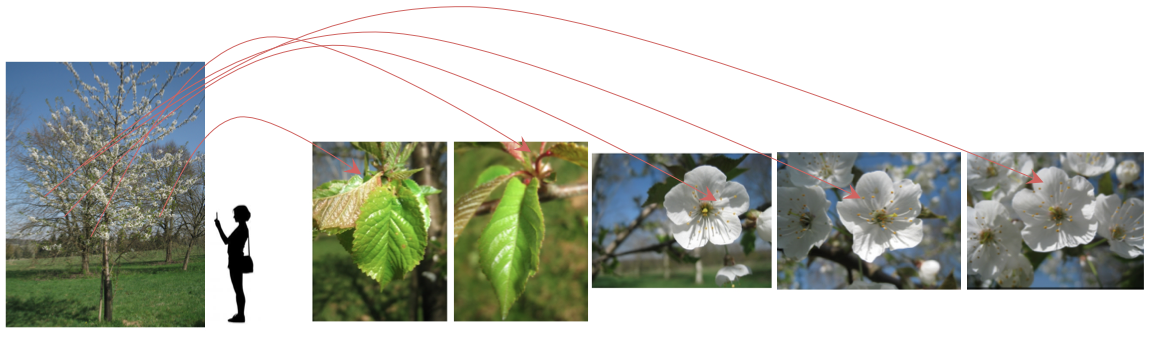
\includegraphics[scale=0.27]{OnePrunus.png}



\end{frame}
%%-----------------------------------------------------------------------------------------

\begin{frame} \frametitle{Project context (2/2)}
%%-----------------------------------------------------------------------------------------
%% Image Indexing
%%-----------------------------------------------------------------------------------------
\begin{block}{Objectives}
    \begin{itemize}
        \item Index image database composed of nature pictures
        \item Adapt XLIM's descriptor to the current image classification
        \item Benchmark results
    \end{itemize}
\end{block}
	
\begin{figure}
	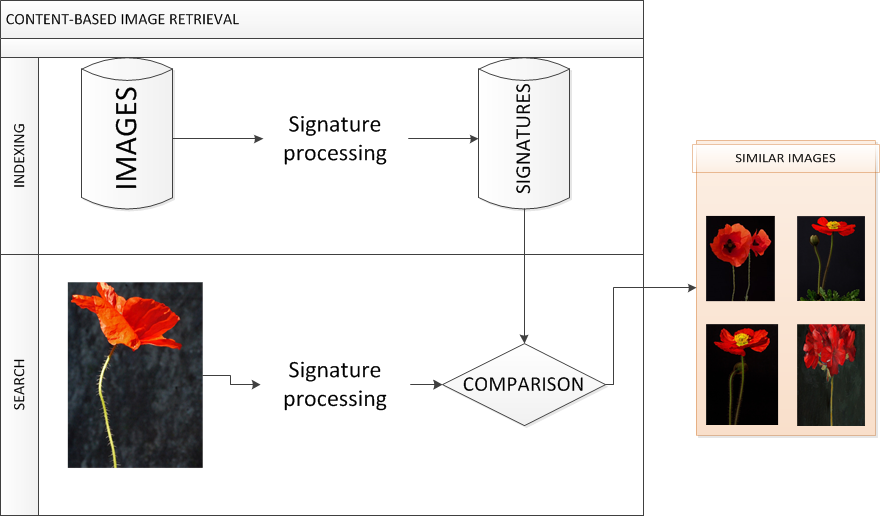
\includegraphics[scale=0.38]{CBIR.png}
\end{figure}

\end{frame}
%%-----------------------------------------------------------------------------------------


%%-----------------------------------------------------------------------------------------
%%-----------------------------------------------------------------------------------------

\begin{frame} \frametitle{Team presentation}
%%-----------------------------------------------------------------------------------------

% Schema demande par mr Richard
\begin{figure}[h]
    \center
    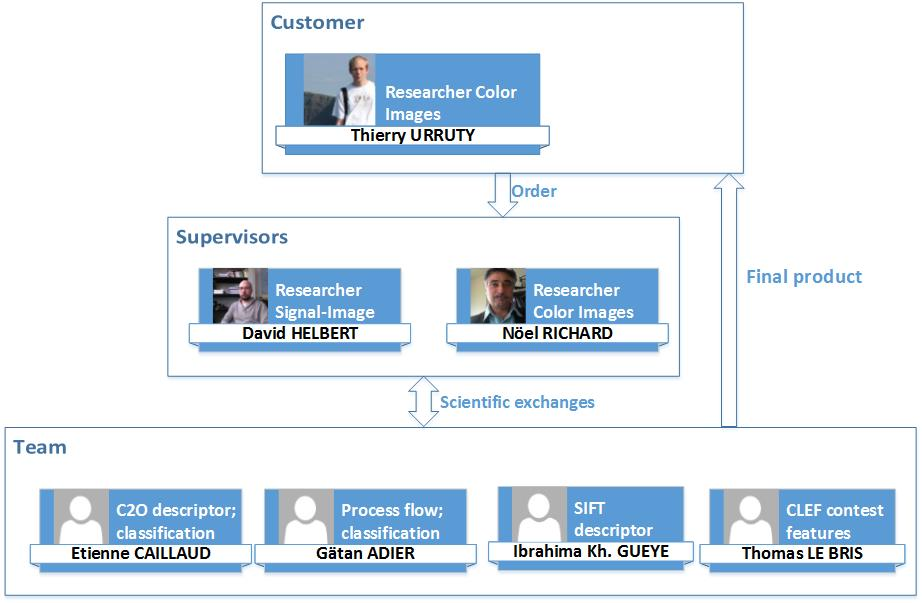
\includegraphics[scale=0.45]{Dessin1.jpg}
    \caption{Team}\label{fig:team}
\end{figure}

\end{frame}
%%-----------------------------------------------------------------------------------------

% A INCLURE CLAIREMENT DANS L'INTRODUCTION
%\begin{frame} \frametitle{User requirement}
%%-----------------------------------------------------------------------------------------

% Parler de la demande de base, ce qui etait convenu avec le client ...

%\begin{itemize}
% \item Design  software programs:\\
%   indexation of  images database,calculate descriptor according to  nature images
%\item Adapt the last up to date designed color and texture attributes to the current image classification
%\item Compare our results (using CLEF challenge metrics)
%\item Provide an abstract of the comparisons and a technical report
%\end{itemize}

%\end{frame}
%%-----------------------------------------------------------------------------------------


\section{Work and results}
\begin{frame} \frametitle{SIFT(1/2)}

\begin{tikzpicture}[remember picture, overlay]
  \node [anchor=north east, inner sep=2pt]  at (current page.north east)
     {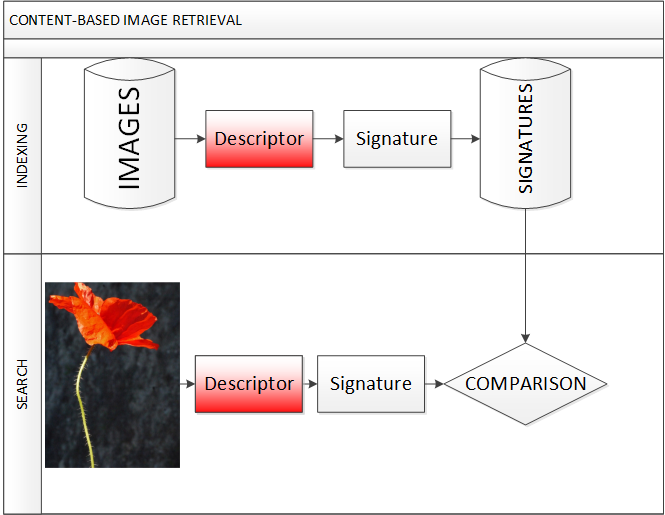
\includegraphics[height=2.5cm]{DescriptorTopImg.png}};
\end{tikzpicture}

Key-points detection (x,y,$\sigma$)


\begin{figure}[htbp]
    \begin{minipage}[c]{.45\linewidth}
      \begin{itemize}

    \item Scale-space extrema detection\\


    \item  Key-point location\\


    \item Orientation assignment\\


    \item key-point descriptor

    \end{itemize}
    \end{minipage}
    \hfill
    \begin{minipage}[c]{.45\linewidth}
      \begin{center}
	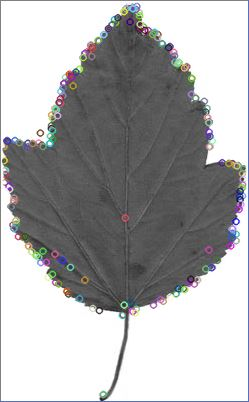
\includegraphics[scale=0.27]{siftKP.jpg}
	\caption{SIFT Keypoints}
	\label{figure:Illustration}
      \end{center}
    \end{minipage}
  \end{figure}





\end{frame}

\begin{frame} \frametitle{SIFT(2/2)}
% Image en haut a droite rapellant l'avancee dans le process flow
\begin{tikzpicture}[remember picture, overlay]
  \node [anchor=north east, inner sep=2pt]  at (current page.north east)
     {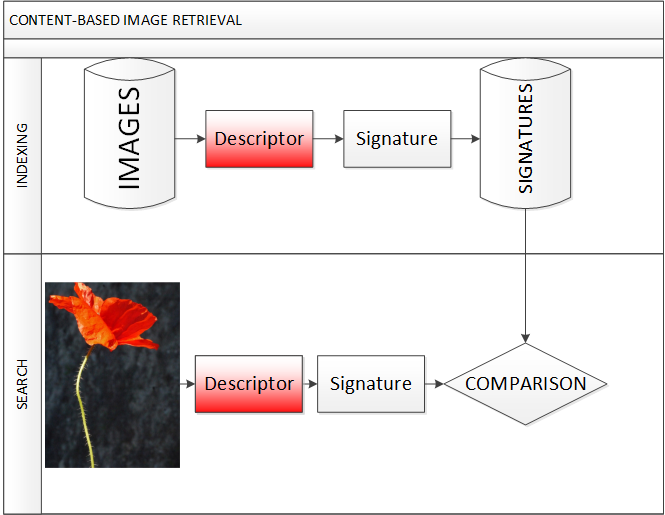
\includegraphics[height=2.5cm]{DescriptorTopImg.png}};
\end{tikzpicture}

\begin{figure}[htbp]
    \begin{minipage}[c]{.45\linewidth}
      \begin{center}
	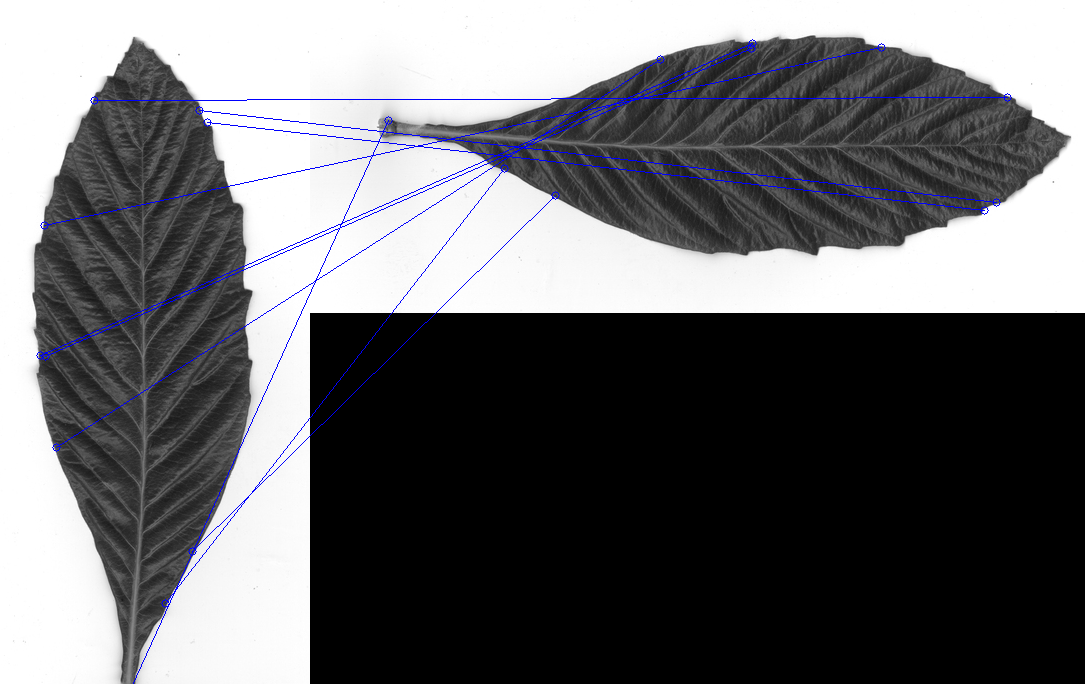
\includegraphics[scale=0.20]{Capture1.png}
	\caption{SIFT Matching for rotation}
	\label{figure:Illustration}
      \end{center}
    \end{minipage}
    \hfill
    \begin{minipage}[c]{.45\linewidth}
      \begin{center}
	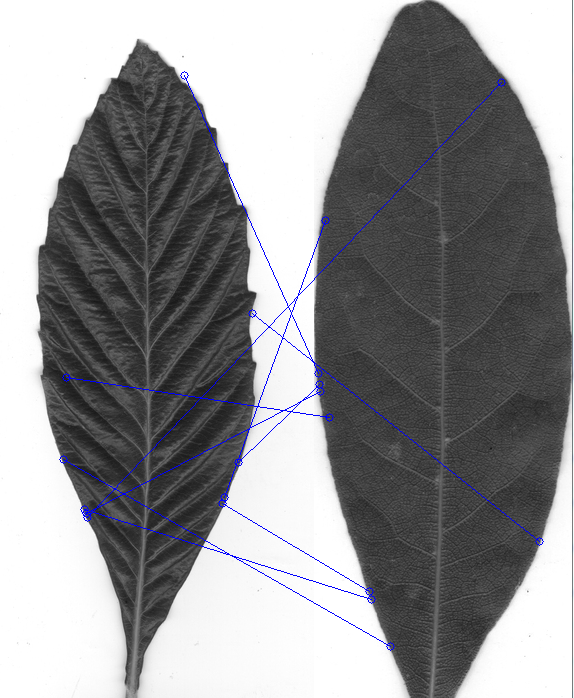
\includegraphics[scale=0.20]{Capture.png}
	\caption{SIFT matching for scale changes}
	\label{figure:Illustration}
      \end{center}
    \end{minipage}
  \end{figure}
\end{frame}



\begin{frame} \frametitle{What about nature images?}
%%-----------------------------------------------------------------------------------------
% Commencer par l'interet des C2O par rapport aux autres descripteurs, (difference entre traitement vectoriel et marginal,...)

% Image en haut a droite rapellant l'avancee dans le process flow
\begin{tikzpicture}[remember picture, overlay]
  \node [anchor=north east, inner sep=2pt]  at (current page.north east)
     {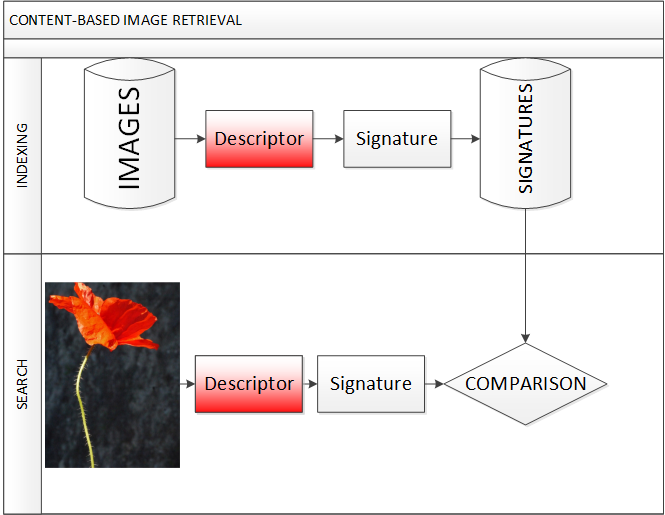
\includegraphics[height=2.5cm]{DescriptorTopImg.png}};
\end{tikzpicture}

\begin{columns}[t]
  \begin{column}{5cm}
  \begin{block}{SIFT}
	\begin{itemize}
		\item Description using orientation of shapes
		\item Natively used on grayscale images
		\item Only marginal methods for color images
		\item Unable to get the texture information from image
	\end{itemize}
  \end{block}
  \end{column}

  \begin{column}{5cm}
  \begin{block}{C$_2$O}
  \begin{itemize}
		\item Description based on color difference
		\item Natively conceived for color images
		\item Take account of the texture information
  \end{itemize}
  \end{block}
  \end{column}
 \end{columns}
\end{frame}
%%-----------------------------------------------------------------------------------------






\begin{frame} \frametitle{C$_2$O (1/2)}
%%-----------------------------------------------------------------------------------------

% Image en haut a droite rapellant l'avancee dans le process flow
\begin{tikzpicture}[remember picture, overlay]
  \node [anchor=north east, inner sep=2pt]  at (current page.north east)
     {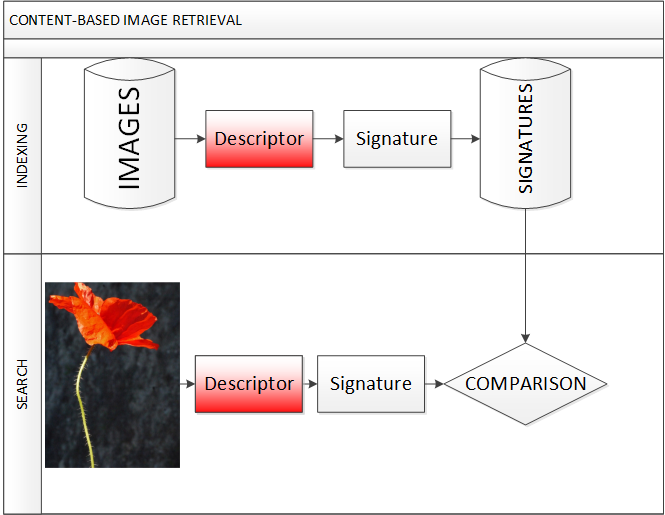
\includegraphics[height=2.5cm]{DescriptorTopImg.png}};
\end{tikzpicture}

% Mettre des exemples de matrice C2O sur des images de la base qui seront parlant !!

\begin{itemize}


\item<1-> The C$_2$O matrix for a poorly textured image :
\only<1> {\begin{figure}[htbp]
    \begin{minipage}[c]{.40\linewidth}
      \begin{center}
    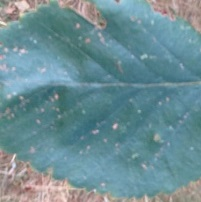
\includegraphics[scale=1.0]{61p.jpg}
    \caption{Image to characterize}
    \label{fig:Sig}
      \end{center}
    \end{minipage}
    \hfill
    \begin{minipage}[c]{.55\linewidth}
      \begin{center}
    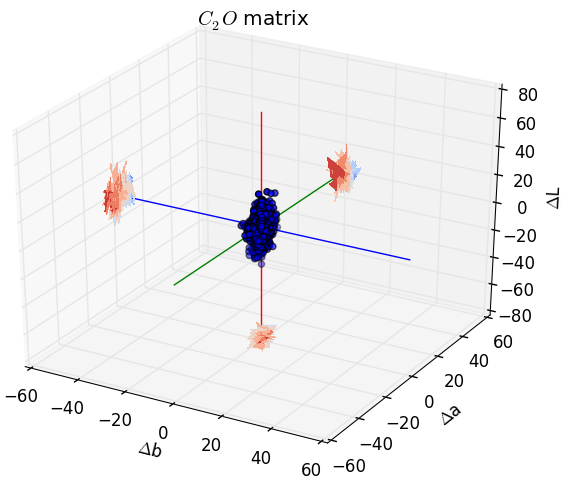
\includegraphics[scale=0.38]{C2OMat61p.png}
    \caption{Signature}
    \label{fig:Sig}
      \end{center}
    \end{minipage}
\end{figure}}
\item<2-> The C$_2$O matrix for a more textured image :
\only<2> {\begin{figure}[htbp]
    \begin{minipage}[c]{.40\linewidth}
      \begin{center}
    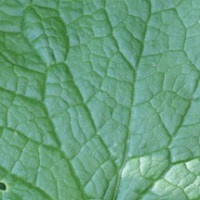
\includegraphics[scale=0.50]{119p.jpg}
    \caption{Image to characterize}
    \label{fig:Sig}
      \end{center}
    \end{minipage}
    \hfill
    \begin{minipage}[c]{.55\linewidth}
      \begin{center}
    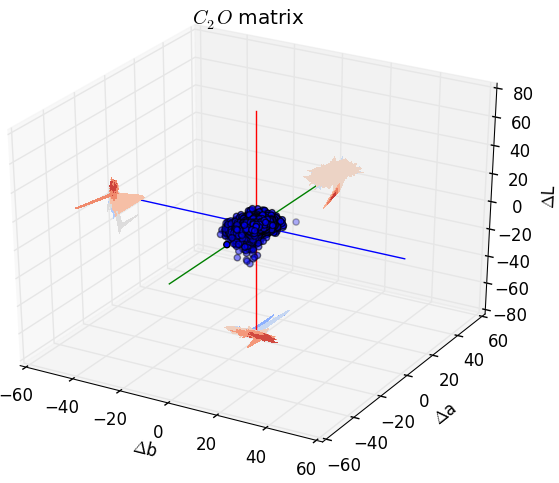
\includegraphics[scale=0.38]{C2OMat119p.png}
    \caption{Signature}
    \label{fig:Sig}
      \end{center}
    \end{minipage}
\end{figure}}
\item<3-> The C$_2$O matrix for a more textured and colored image :
\only<3> {\begin{figure}[htbp]
    \begin{minipage}[c]{.40\linewidth}
      \begin{center}
    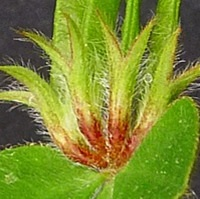
\includegraphics[scale=0.50]{97p.jpg}
    \caption{Image to characterize}
    \label{fig:Sig}
      \end{center}
    \end{minipage}
    \hfill
    \begin{minipage}[c]{.55\linewidth}
      \begin{center}
    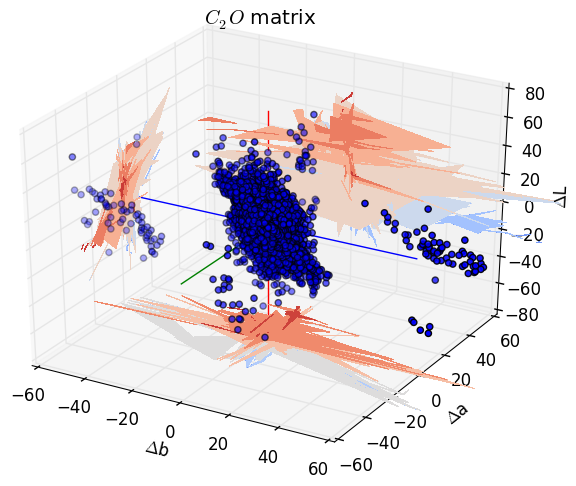
\includegraphics[scale=0.38]{C2OMat97p.png}
    \caption{Signature}
    \label{fig:Sig}
      \end{center}
    \end{minipage}
\end{figure}}

\end{itemize}

\end{frame}
%%-----------------------------------------------------------------------------------------


\begin{frame} \frametitle{C$_2$O (2/2)}
%%-----------------------------------------------------------------------------------------

% Mettre en petit en haut l'illustration coords spheriques et montrer les signatures correspondant aux matrices


% Image en haut a droite rapellant l'avancee dans le process flow
\begin{tikzpicture}[remember picture, overlay]
  \node [anchor=north east, inner sep=2pt]  at (current page.north east)
     {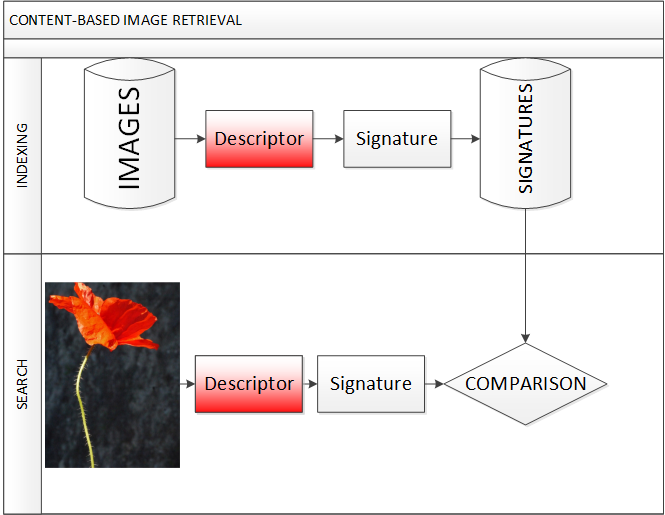
\includegraphics[height=2.5cm]{DescriptorTopImg.png}};
\end{tikzpicture}


\begin{tikzpicture}[remember picture, overlay]
  \node [anchor=south east, inner sep=0pt]  at (current page.south east)
     {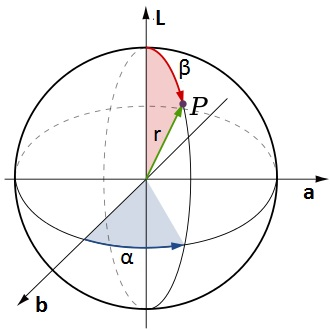
\includegraphics[height=2.5cm]{Spherical_Coordinates}};
\end{tikzpicture}



\begin{itemize}
\item<1-> The C$_2$O signature for a poorly textured image :
\only<1> {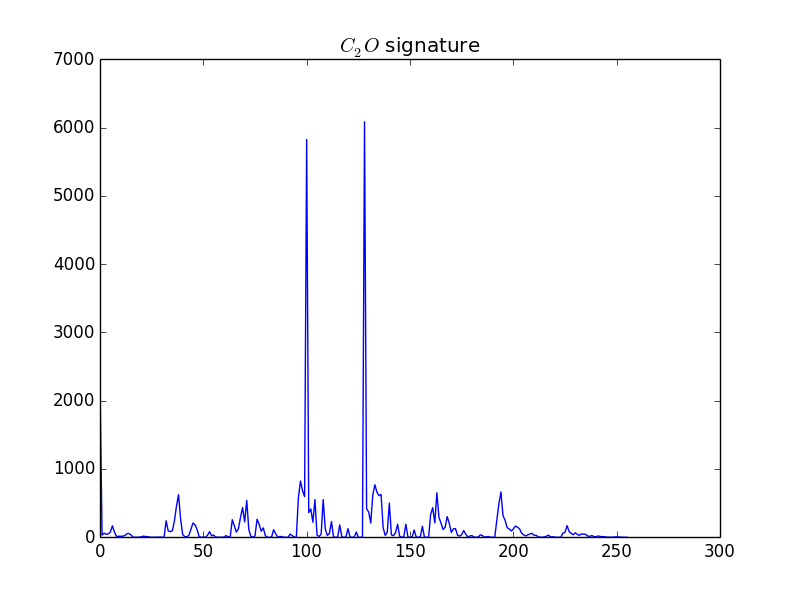
\includegraphics[height=4cm]{C2OSig61p.png}}
\item<2-> The C$_2$O signature for a more textured image :
\only<2> {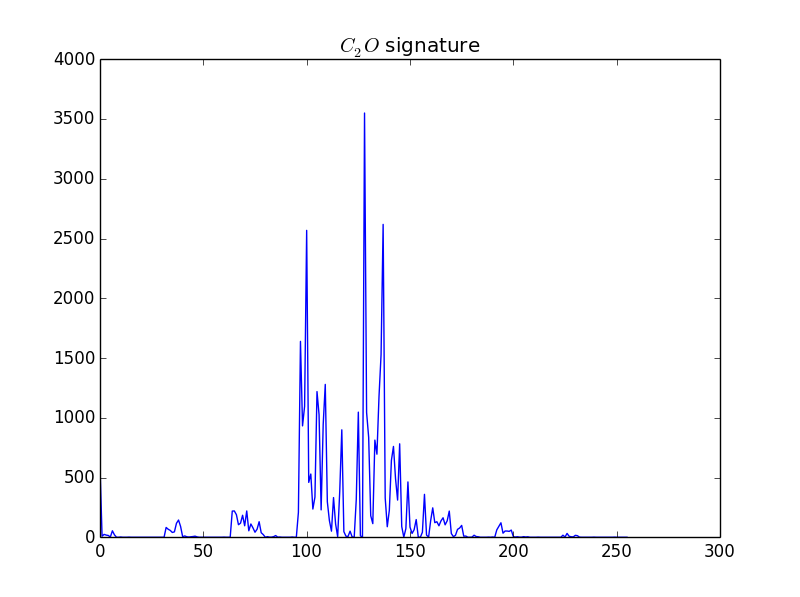
\includegraphics[height=4cm]{C2OSig119p.png}}
\item<3-> The C$_2$O signature for a more textured and colored image :
\only<3> {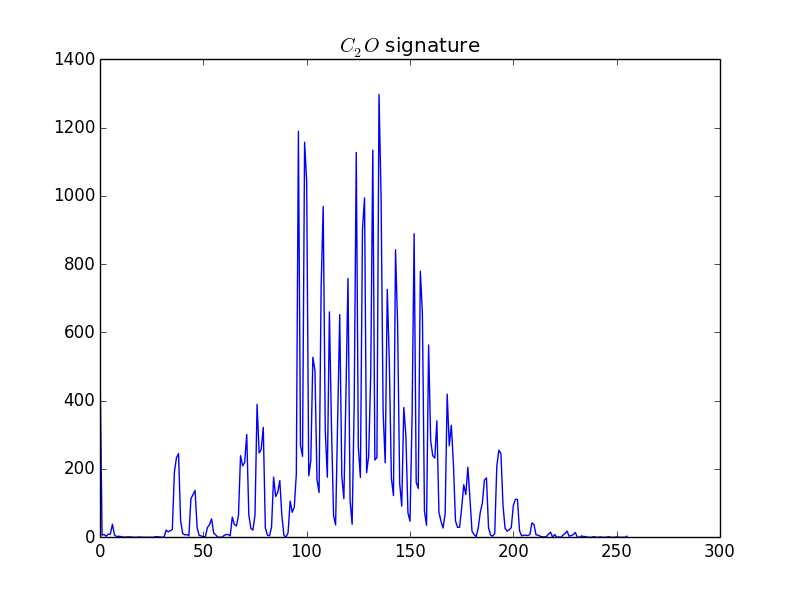
\includegraphics[height=4cm]{C2OSig97p.png}}

\end{itemize}



\end{frame}
%%-----------------------------------------------------------------------------------------




\begin{frame} \frametitle{Bag of word (1/2)}
%%-----------------------------------------------------------------------------------------

% Image en haut a droite rapellant l'avancee dans le process flow
\begin{tikzpicture}[remember picture, overlay]
  \node [anchor=north east, inner sep=2pt]  at (current page.north east)
     {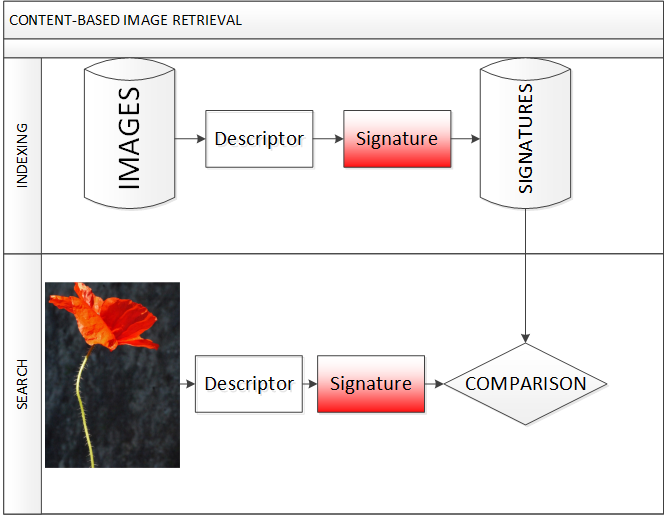
\includegraphics[height=2.5cm]{SignatureTopImg.png}};
\end{tikzpicture}

Reducing the number of points (100 in our case).

\begin{itemize}
    \item K-means
    \begin{itemize}
        \item Attribute the vectors to centroid vectors.
    \end{itemize}
\end{itemize}

\begin{figure}[h]
        \centering
        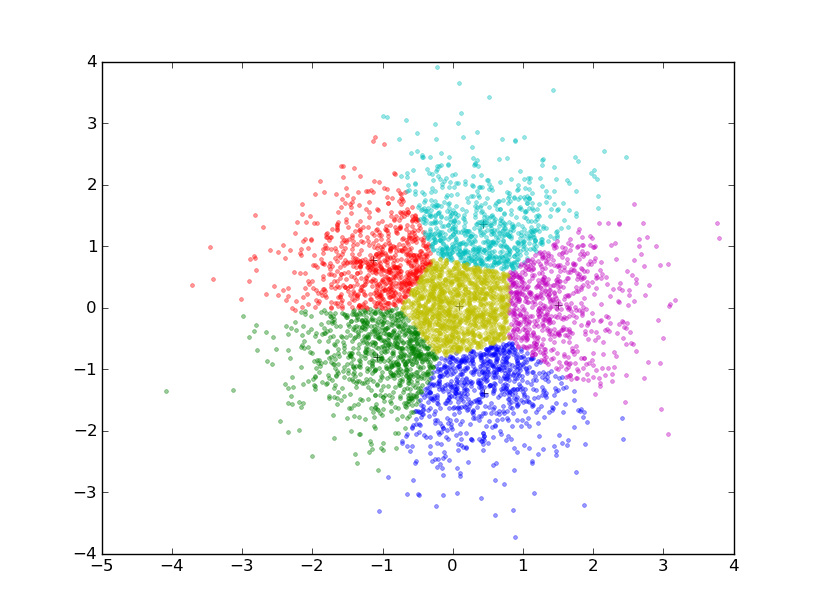
\includegraphics[scale=0.25]{k6n5000.png}
        \caption{K-means}
        \label{fig:kmeans}
    \end{figure}

\end{frame}
%%-----------------------------------------------------------------------------------------

\begin{frame} \frametitle{Bag of word (2/2)}
%%-----------------------------------------------------------------------------------------

% Image en haut a droite rapellant l'avancee dans le process flow
\begin{tikzpicture}[remember picture, overlay]
  \node [anchor=north east, inner sep=2pt]  at (current page.north east)
     {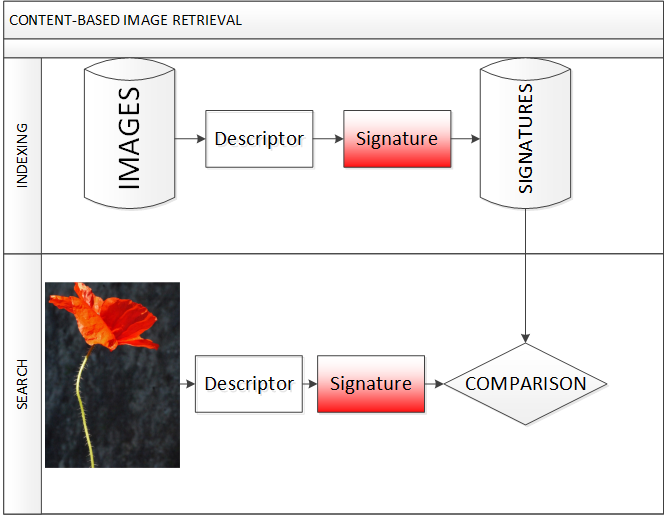
\includegraphics[height=2.5cm]{SignatureTopImg.png}};
\end{tikzpicture}

\begin{itemize}
    \item Signature
    \begin{itemize}
        \item Design histogram in function of assignment of the vectors.
    \end{itemize}
\end{itemize}

\begin{figure}[htbp]
    \begin{minipage}[c]{.45\linewidth}
      \begin{center}
    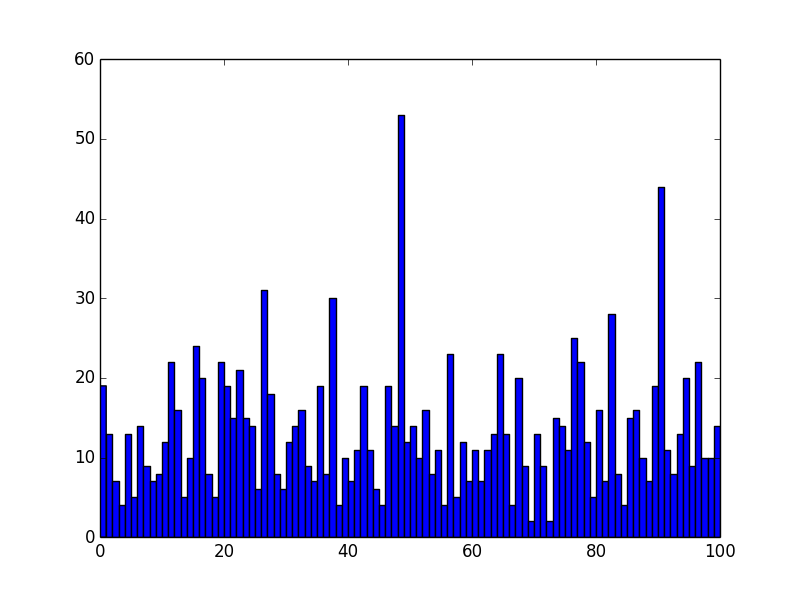
\includegraphics[scale=0.20]{131_sig.png}
    \caption{Signature 100 words - 1}
    \label{fig:image4}
      \end{center}
    \end{minipage}
    \hfill
    \begin{minipage}[c]{.45\linewidth}
      \begin{center}
    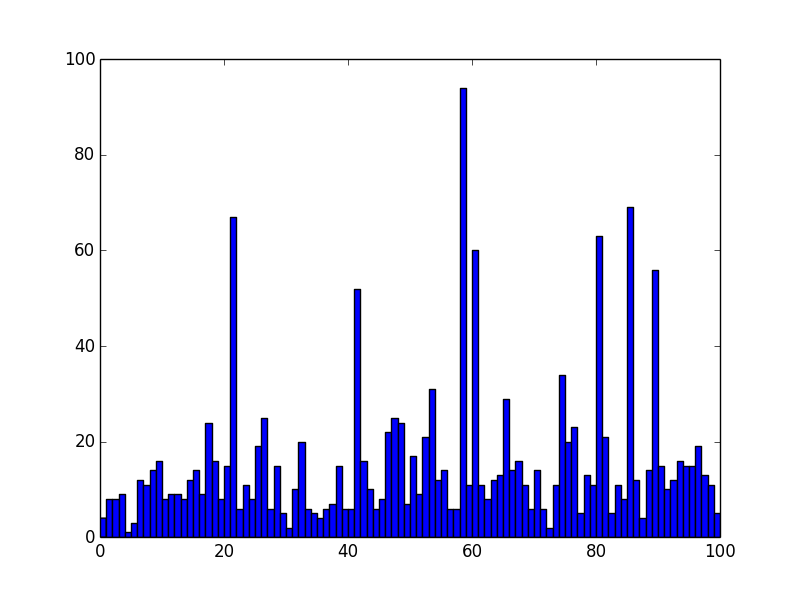
\includegraphics[scale=0.20]{132_sig.png}
    \caption{Signature 100 words - 2}
    \label{fig:image5}
      \end{center}
    \end{minipage}
\end{figure}


\end{frame}
%%-----------------------------------------------------------------------------------------


\begin{frame}\frametitle{K-nn(1/2)}

% Image en haut a droite rapellant l'avancee dans le process flow
\begin{tikzpicture}[remember picture, overlay]
  \node [anchor=north east, inner sep=2pt]  at (current page.north east)
     {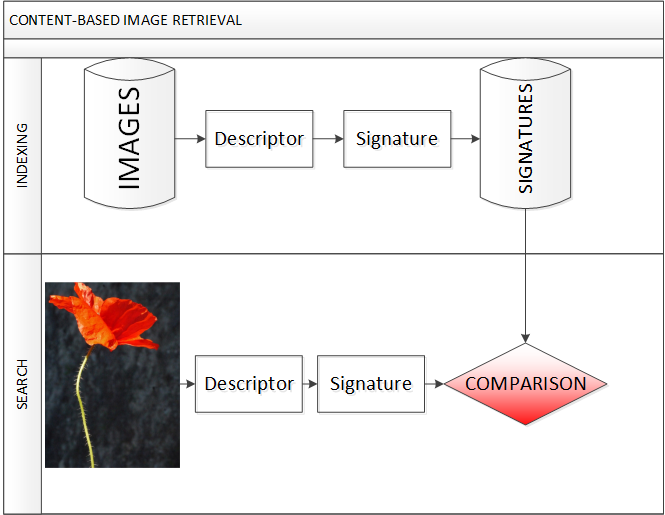
\includegraphics[height=2.5cm]{knnTopImg.png}};
\end{tikzpicture}

- The k nearest neighbor method

\begin{itemize}
\item<1-> Comparison to the dictionary .
\only<1> {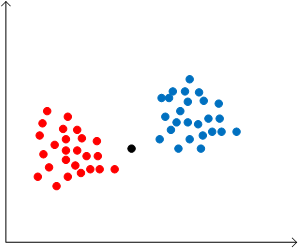
\includegraphics[height=4.2cm]{knnwc.png}} % Changer l'image
\only<2> {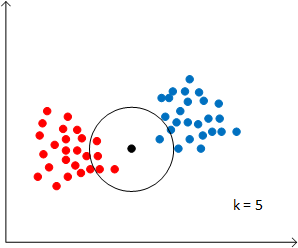
\includegraphics[height=4cm]{knnac.png}
\item 4 Occurrences of {the \color{red} red} class
\item 1 occurrence of {the \color{blue} blue} class
\item The new point is attributed to {the \color{red} red} class}
\end{itemize}

\end{frame}

\begin{frame}\frametitle{K-nn(2/2)}

% Image en haut a droite rapellant l'avancee dans le process flow
\begin{tikzpicture}[remember picture, overlay]
  \node [anchor=north east, inner sep=2pt]  at (current page.north east)
     {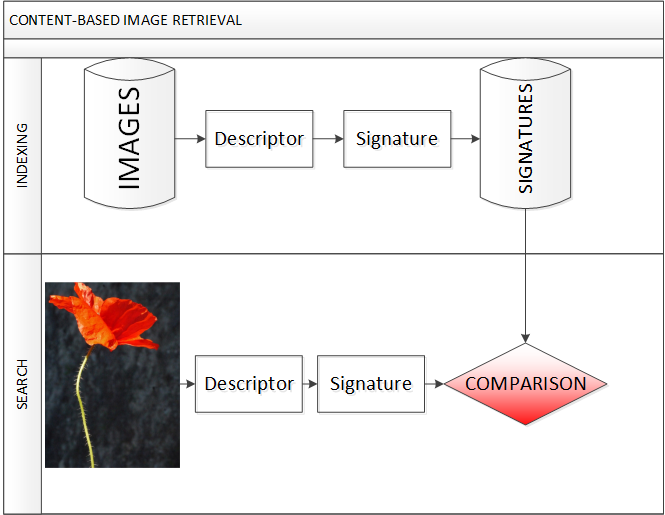
\includegraphics[height=2.5cm]{knnTopImg.png}};
\end{tikzpicture}

- Application for image classification

\begin{itemize}
\item More complex data.
\item Distances on signature vectors extracted from the K-mean method.
\item One most adapted distance type for each descriptor .
\end{itemize}

\end{frame}



\begin{frame} \frametitle{Results (1/2)}

\begin{itemize}
    \item Reduce data-base of 100 images composed of only 4 species.
\end{itemize}

  \begin{figure}[htbp]
    \begin{minipage}[c]{.45\linewidth}
      \begin{center}
	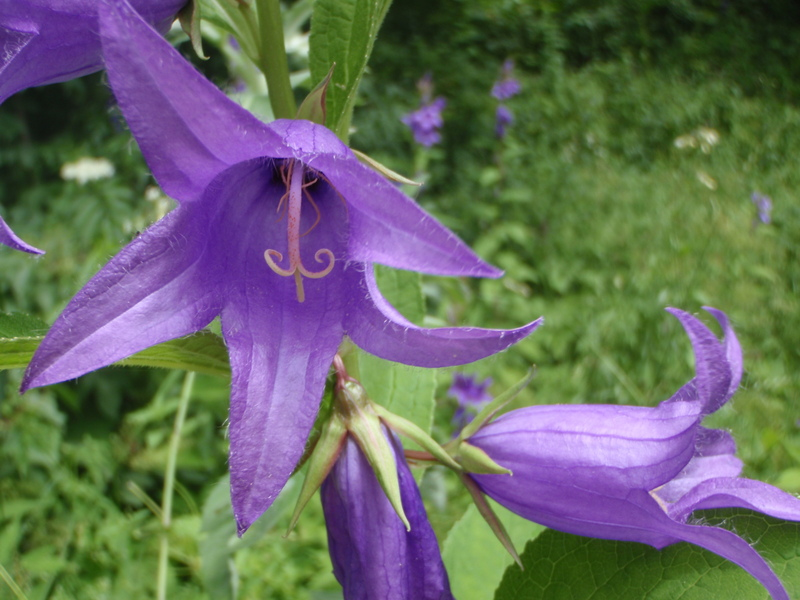
\includegraphics[scale=0.40]{63.jpg}
	\caption{First specie}
	\label{fig:image4}
      \end{center}
    \end{minipage}
    \hfill
    \begin{minipage}[c]{.45\linewidth}
      \begin{center}
	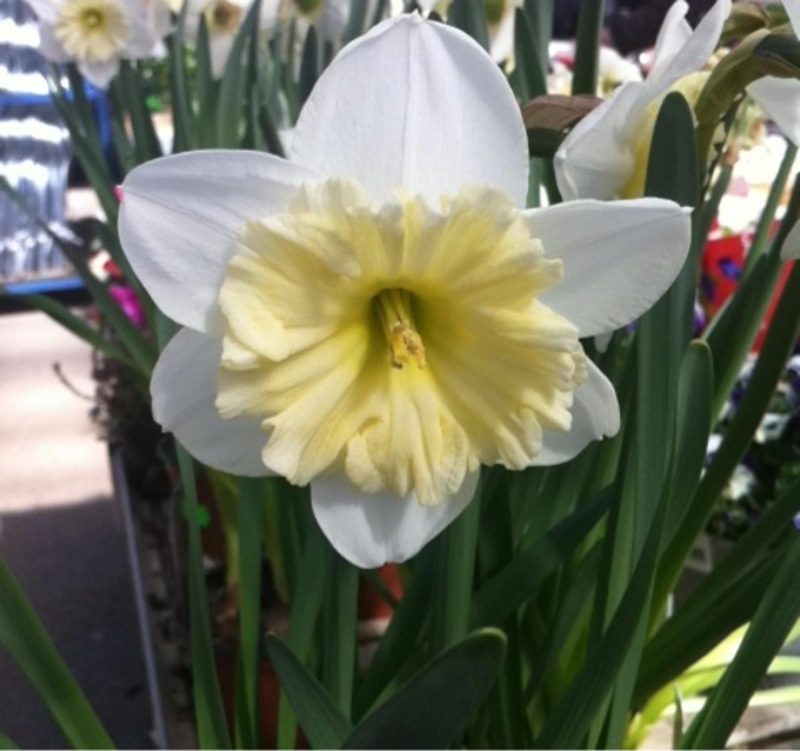
\includegraphics[scale=0.08]{2391.jpg}
	\caption{Second specie}
	\label{fig:image5}
      \end{center}
    \end{minipage}
  \end{figure}


  \begin{figure}[htbp]
    \begin{minipage}[c]{.45\linewidth}
      \begin{center}
	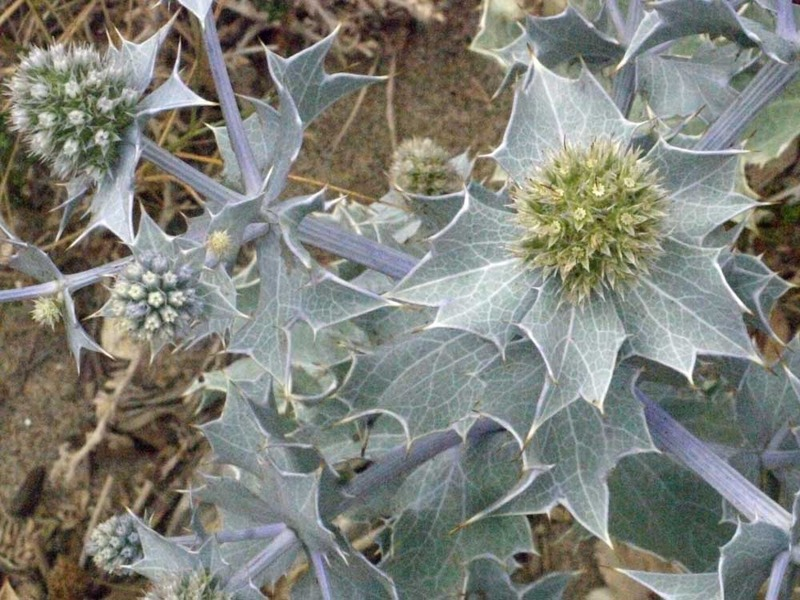
\includegraphics[scale=0.20]{4971.jpg}
	\caption{Third specie}
	\label{fig:image6}
      \end{center}
    \end{minipage}
    \hfill
    \begin{minipage}[c]{.45\linewidth}
      \begin{center}
	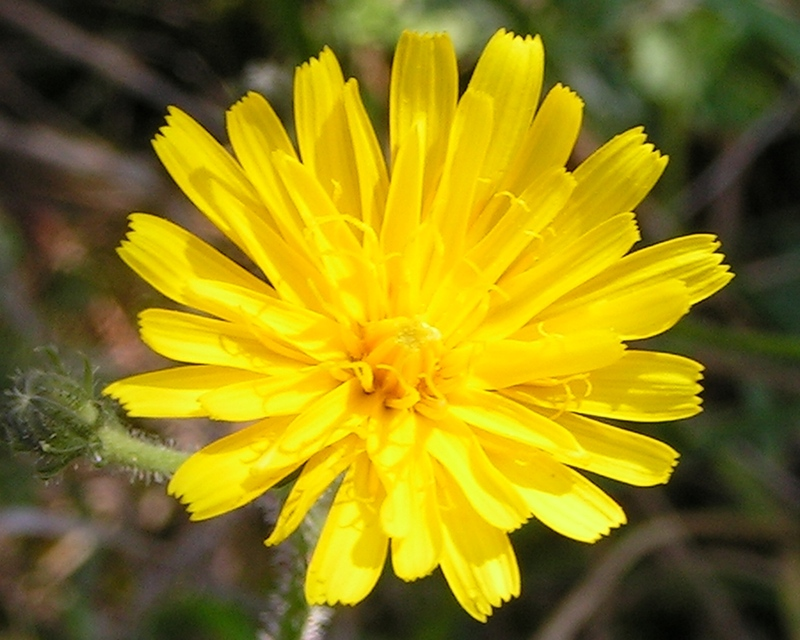
\includegraphics[scale=0.08]{21604.jpg}
	\caption{Fourth specie}
	\label{fig:image7}
      \end{center}
    \end{minipage}
  \end{figure}

\end{frame}


\begin{frame} \frametitle{Results (2/2)}
%%-----------------------------------------------------------------------------------------
\begin{itemize}
    \item Compare the two descriptors SIFT and C$_2$O.
\end{itemize}

\begin{figure}[htbp]
    \resizebox{3.5cm}{!}{
    \begin{minipage}[c]{.55\linewidth}
      \begin{center}
        \begin{table}[H]
        \centering
        \caption{SIFT result}
        \label{tab1}
        \begin{tabular}{|l|l|l|l|l|}
        \hline
        ID & Training Base & Test Base & Correct & Accuracy \\ \hline
        173 & 17 & 8 & 4 & 50\% \\ \hline
        1102 & 22 & 3 & 1 &\cellcolor{red!75} 33\% \\ \hline
        1889 & 16 & 9 & 1 & 11\% \\ \hline
        2717 & 15 & 10 & 7 &\cellcolor{red!75} 70\% \\ \hline
        Total & 70 & 30 & 9 & / \\ \hline
        \end{tabular}
        \end{table}
      \end{center}
    \end{minipage}}

    \resizebox{3.5cm}{!}{
    \begin{minipage}[c]{.55\linewidth}
      \begin{center}
            \begin{table}[H]
            \caption{C$_2$O result}
            \label{tab2}
            \begin{tabular}{|l|l|l|l|l|}
            \hline
            ID & Training Base & Test Base & Correct & Accuracy \\ \hline
            173 & 17 & 8 & 1 & 12.5\% \\ \hline
            1102 & 22 & 3 & 1 &\cellcolor{red!75} 33\% \\ \hline
            1889 & 16 & 9 & 0 & 0\% \\ \hline
            2717 & 15 & 10 & 7 &\cellcolor{red!75} 70\% \\ \hline
            Total & 70 & 30 & 9 & / \\ \hline
            \end{tabular}
            \end{table}
      \end{center}
    \end{minipage}}
\end{figure}

\end{frame}
%%-----------------------------------------------------------------------------------------

\begin{frame} \frametitle{Discussion}

\begin{itemize}
    \item Classification
    \vspace{0.3cm}
    \begin{itemize}
        \item To much reducing on the K-means (100 words).
        \vspace{0.15cm}
        \item Euclidean distance not the most efficient or adapt.
    \end{itemize}
    \vspace{0.7cm}
    \item C$_2$O
    \vspace{0.3cm}
    \begin{itemize}
        \item The concatenation way is not optimal.
        \item Parameters D, alpha, and beta has to be discussed regarding to the images.
    \end{itemize}
\end{itemize}
\end{frame}
%%-----------------------------------------------------------------------------------------


%%-----------------------------------------------------------------------------------------
\section{Project management}
%%-----------------------------------------------------------------------------------------




\begin{frame} \frametitle{Scheduling (1/2)}
%%-----------------------------------------------------------------------------------------
% Montrer le passage d'un gantt a un backlog produit, => mettre l'accent sur la modification du gantt sans modification du backlog notable

\begin{itemize}
\item The forecast Gantt chart  :
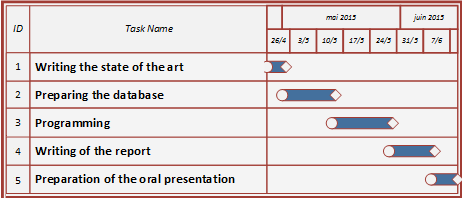
\includegraphics[scale=0.80]{GanttPrez.png}
\item All time affectation done before the beginning of the project
\item Rarely respected in important project
\end{itemize}

\end{frame}
%%-----------------------------------------------------------------------------------------


\begin{frame} \frametitle{Scheduling (2/2)}
%%-----------------------------------------------------------------------------------------
% Montrer le passage d'un gantt a un backlog produit, => mettre l'accent sur la modification du gantt sans modification du backlog notable


\begin{itemize}
\item The project backlog  :
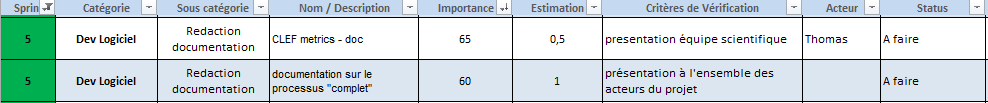
\includegraphics[scale=0.40]{backlog.png}
\item Division of each main task in subtasks
\item Time attribution for each subtask
\item Tasks sorted by priority
\item Each subtask attributed to team member
\item Allow to change the affectation of a task
\item Weekly time affectation : could be adapted to unforeseen
\end{itemize}


\end{frame}
%%-----------------------------------------------------------------------------------------




%%-----------------------------------------------------------------------------------------
\section{Conclusion}
%%-----------------------------------------------------------------------------------------

\begin{frame} \frametitle{Sum-up of the situation}
%%-----------------------------------------------------------------------------------------

\begin{columns}[t]
  \begin{column}{5cm}
  \begin{block}{Starting objectives}
	\begin{itemize}
		\item SIFT tests
		\item C2O programming
		\item classification programming
		\item Code optimizing for speed
		\item parallelization
	\end{itemize}
  \end{block}
  \end{column}

  \begin{column}{5cm}
  \begin{block}{Ending situation}
  \begin{itemize}
		\item SIFT tests
		\item C2O programming
		\item classification programming
  \end{itemize}
  \end{block}
  \end{column}
 \end{columns}

\begin{alertblock}{Issues}
	\begin{itemize}
		\item C2O concatenation order
		\item distance calculation
	\end{itemize}	
\end{alertblock}
\end{frame}



\begin{frame}\frametitle{Personal conclusion}
%----------------------------------------------------------------------------------------
\begin{columns}[t]
  \begin{column}{5cm}
    \begin{block}{Personal gains}
      \begin{itemize}
            \item New way to organize teamwork
            \item Technical knowledge
            \item Contest participation context
            \item Code management on a project scale
      \end{itemize}
    \end{block}
  \end{column}

  \begin{column}{5cm}
  \begin{block}{Perspectives}
  \begin{itemize}
        \item Fixing technical issues
        \item Test on the whole database
        \item Classification programming
  \end{itemize}
  \end{block}
  \end{column}
\end{columns}


\end{frame}


\section{}
\begin{frame}\frametitle{}
%%-----------------------------------------------------------------------------------------
    \begin{center}
        \huge Thank you for attention
    \end{center}
\end{frame}
%%-----------------------------------------------------------------------------------------


\end{document}

